

\actTitle{Worksheet 1.1}

\noindent \textbf{Instructions:}  Work together in groups of  3 or 4 to complete the following problems.


\begin{enumerate}
\item The points $ABC$ form a triangle.
\begin{enumerate}
\item Plot $A(-1,2),B(3,0) , C(4,2), $ and draw the triangle on the graph below.\\

 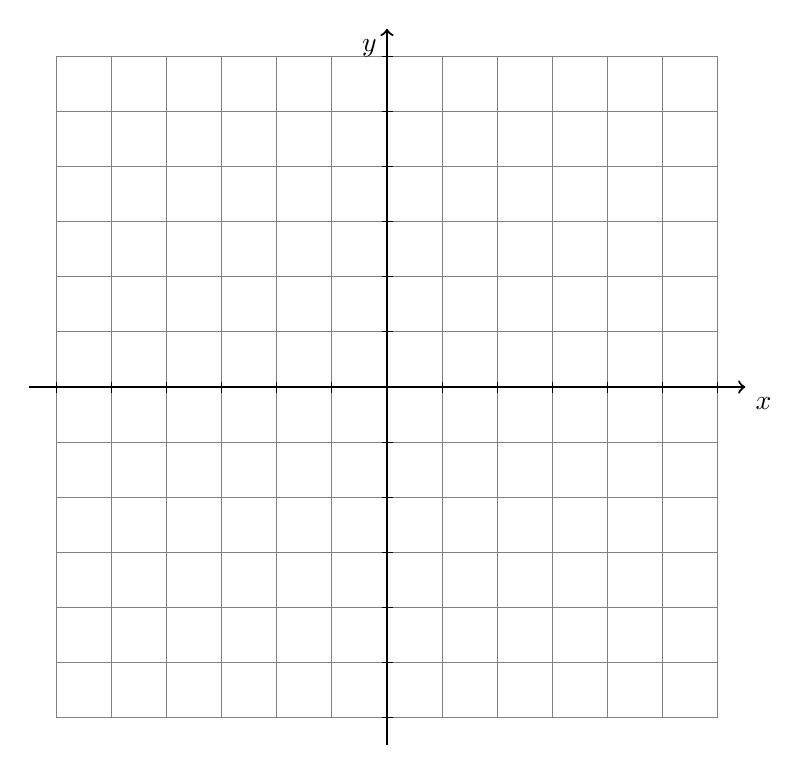
\begin{tikzpicture}[y=.7cm, x=.7cm,font=\sffamily]
    %% ticks
    \draw[step = 1, gray] (-6,-6) grid (6,6);
    %% axis
    \draw[thick,->] (-6.5,0) -- coordinate (x axis mid) (6.5,0) node[anchor = north west] {$x$};
    \draw[thick,->] (0,-6.5) -- coordinate (y axis mid) (0,6.5) node[anchor = north east] {$y$};
    \foreach \y in {-6,-5,...,-1,1,2,...,6} {
      \draw (2pt, \y) -- (-2pt, \y);
    }
    \foreach \x in {-6,-5,...,-1,1,2,...,6} {
      \draw (\x,2pt) -- (\x,-2pt);
    }

  \end{tikzpicture}

\item Find the perimeter of the triangle.\vfill
\item Is the triangle a right triangle?  Show work to support your answer.\\[1in]
\end{enumerate}


\newpage


\item Find the $x$ and $y$ intercepts of the following equations.
\begin{enumerate}
\item $x^2+y=9$
\vfill
\item $y=|x+4|-3$
\end{enumerate}
%\item Determine the distance between the points $A(-3, 4)$ and  $C(4, -8)$. \\[2.5in]
\vfill

\newpage

\item Use the given problem solving process below to determine all points lying on the $y$-axis that are 5 units away from the point $(4,-2)$.  As a group, write your complete solution on the board. 


\begin{boxthm}
{\bf Problem Solving Process}
\begin{enumerate}
\item Re-read the problem.
\item Determine what the problem is asking for along with the format of that answer.
\item Circle/Underline the important components of the problem.
\item Determine the topics/concepts being assessed.
\item Write down relevant formulas, definitions, and equations.
\item Discuss your ideas with your group.
\item Solve the problem and verify that your solution answers the question in the correct format.
\end{enumerate}

\end{boxthm}
\vfill
\newpage

\item Use the following parts to find all points on the line $y=2x$ that are 5 units away from $P(-1,3)$.  
\begin{enumerate}
\item Find the points $(x,y)$ on the line $y=2x$ for $x=1, -2,$ and $5$.
\vfill
\item What if we didn't know the value of $x$?  Write an ordered pair formula that works for every point on the line $y=2x$?\vfill
\item Use part (b) to find all points on the line $y=2x$ that are 5 units away from $P(-1,3)$. 
\vfill
\vfill
\vfill
\end{enumerate}
\newpage





\end{enumerate}













